\documentclass[a4paper,11pt]{article}
\usepackage{hometask}
\usepackage{amssymb}
\usepackage{graphicx}
\usepackage{overpic}
\usepackage{xcolor}

\setlength{\parindent}{0pt}
\setlength{\parskip}{5pt}
\setlength{\headheight}{24pt}
\graphicspath{{figures/}}

\begin{document}

{\large\bfseries 1-1.} Переобозначим $t_r(I) \to t(I,r)$, $I\in\mathcal{I}$, $r\in R$.
Для простоты положим, что $|\mathcal{I}|<+\infty$ и $|R|<+\infty$.
Тогда,
\[
M_r[t(I,r)]=\frac{1}{|R|}\sum_R t(I,r),
\qquad
M_r[\max t(I,r)]=\frac{1}{|R|}\sum_R\max_{\mathcal{I}} t(I,r).
\]
Теперь достаточно сравнить
\[
A\sim\max_{\mathcal{I}}\sum_R t(I,r)
\qquad\text{и}\qquad
B\sim\sum_R\max_{\mathcal{I}} t(I,r).
\]
Представим это в виде таблицы:
\begin{center}
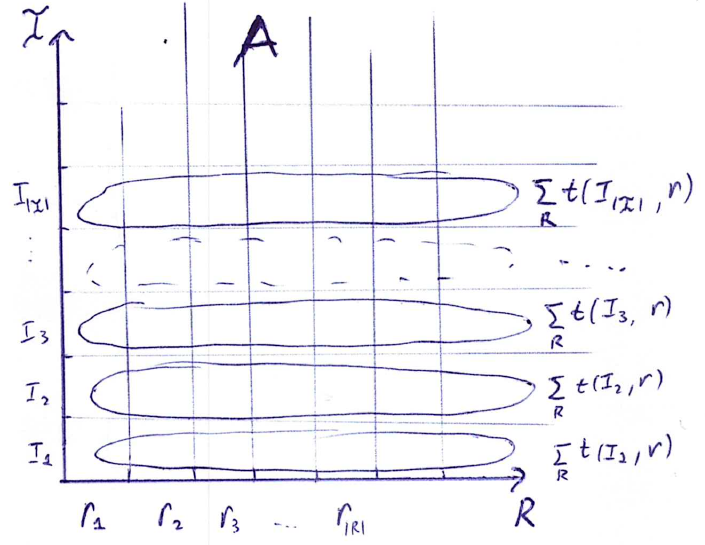
\includegraphics[width=.53\textwidth]{1-1-a.png}\hfill
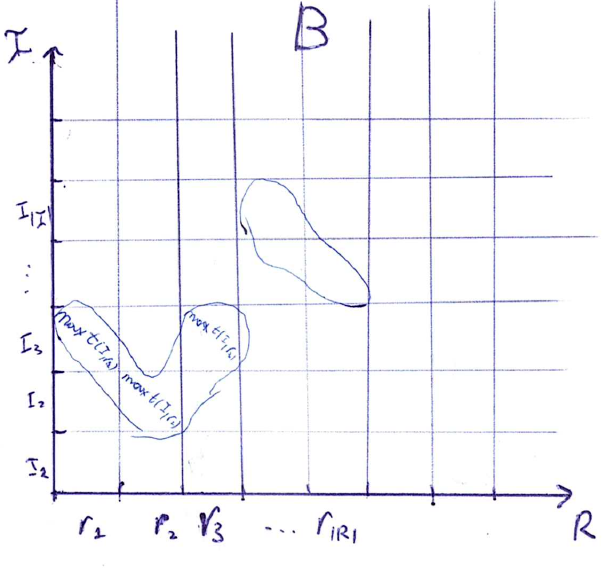
\includegraphics[width=.46\textwidth]{1-1-b.png}
\end{center}
Из рисунков ясно, что $B\geq A$, т.\,к. каждое слагаемое в $B$ $\geq$ чем в $A$.
Распишем подробнее. Пусть
\begin{align*}
A&\sim\max_{\mathcal{I}}\sum_R t(I,r)=\sum_R t(I_m,r)={}\\
&=t(I_m,r_1)+t(I_m,r_2)+\dots+t(I_m,r_{|R|})\\
&\leq t(I_{m_1},r_1)+t(I_{m_2},r_2)+\dots+t(I_{m_{|R|}},r_{|R|})
=\sum_R\max_{\mathcal{I}}t(I,r)\sim B.
\end{align*}

\newpage

{\large\bfseries 1-2.} $g(n)=n$.

Для определенности будем считать, что корень дерева находится на высоте 1, и $g(1)=1$ (сразу лист).

а) Докажем, что $g(n)\geq n$.
Действительно, если у нас есть путь из $(n-2)$ сравнений (и $+1$ лист в конце),
то граф сравнений будет не связным:

\begin{center}
\begin{minipage}{.34\textwidth}
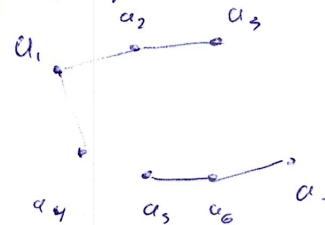
\includegraphics[width=\linewidth]{1-2-graph.png}
\end{minipage}\hfill
\begin{minipage}{.63\textwidth}
$\leftarrow$ вершины --- индексы массива,
ребра --- отношения сравнений, встречающихся на нашем пути длины $n-1$.
\end{minipage}
\end{center}

Граф может быть связным только если ребер $\geq n-1$.
Возьмем произвольный вход $A$, который идет по такому пути (он $\exists$, т.\,к. вершина достижима).
Возьмем его два поднабора индексов $X$, $Y$, соответствующих разным компонентам связности.
Заметим, что по построению, следующие входы обязаны выдавать одинаковый результат:
\[
\begin{cases}
A=\{A_x;A_y\},\\
B=\{A_x;A_y+L\},\\
C=\{A_x;A_y-L\}.
\end{cases}
\]
Где $L$ --- какое-нибудь большое число, например $L=\sum|a_i|$.
Но это невозможно, т.\,к. $B$ и $C$ гарантированно имеют разные перестановки:
\[
A_y+L\succcurlyeq A_x,\qquad A_y-L\preccurlyeq A_x.
\]

б) Для $g(n)=n$ достаточно взять такую ветку и достроить ее до корректного дерева:
\begin{center}
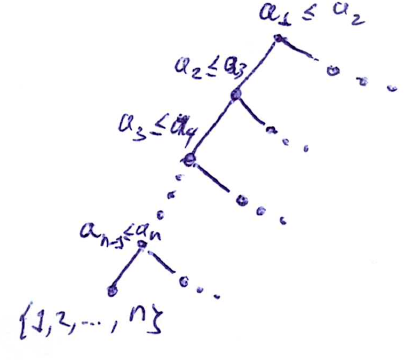
\includegraphics[width=.40\textwidth]{1-2-tree.png}
\end{center}

\newpage

{\large\bfseries 1-3.}
\begin{center}
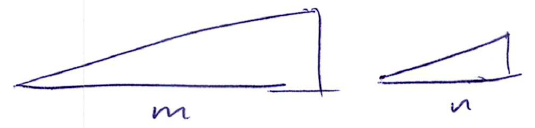
\includegraphics[width=.48\textwidth]{1-3.png}
\end{center}
Заметим, что для произвольного входа, минимальное число возможных перестановок
на выходе решающего дерева $=\dfrac{(m+n)!}{m!\,n!}$.
\[
\begin{aligned}
\leftarrow\quad &(m+n)!\text{ --- число перестановок общего массива},\\
&m!\,n!\text{ --- поправка на то, что 2 части изначально упорядочены}.
\end{aligned}
\]
Тогда, минимальное число сравнений $\sim\log_2\dfrac{(m+n)!}{m!\,n!}$.
\[
\frac{(m+n)!}{m!\,n!}
=\frac{(m+1)\dots(m+n)}{n!}
\geq\frac{(m+1)\dots(m+n)}{n^{n+1}}
\geq\frac{m^n}{n^{n+1}}\quad\Rightarrow
\]
\[
\log_2\left(\frac{(m+n)!}{m!\,n!}\right)
\geq\log_2\frac{m^n}{n^n\cdot n}
=n\log_2\frac{m}{n}-\log_2 n
=\Omega\left(n\log\frac{m}{n}\right).
\]

\newpage
{\large\bfseries 1-4.}
$\displaystyle\min_{A\in\mathcal{A}}M_I f(A,I)\leq\max_{I\in\mathcal{I}}M_A f(A,I)$.
\[
M_I f(A,I)=\sum_{\mathcal{I}}P_{\mathcal{I}}(I)f(A,I);
\qquad M_A f(A,I)=\sum_{\mathcal{A}}P_{\mathcal{A}}(I)f(A,I).
\]
Рассмотрим матрицу
\[
F=\begin{pmatrix}
f(A_1,I_1)&\dots&f(A_{|\mathcal{A}|},I_1)\\
\vdots&\ddots&\vdots\\
f(A_1,I_{|\mathcal{I}|})&\dots&f(A_{|\mathcal{A}|},I_{|\mathcal{I}|})
\end{pmatrix},
\]
\[
P_{\mathcal{I}}=\begin{pmatrix}P_{\mathcal{I}}(I_1)\\\vdots\\P_{\mathcal{I}}(I_{|\mathcal{I}|})\end{pmatrix},
\qquad
P_{\mathcal{A}}=\begin{pmatrix}P_{\mathcal{A}}(A_1)\\\vdots\\P_{\mathcal{A}}(A_{|\mathcal{A}|})\end{pmatrix},
\qquad
\sum P_{\mathcal{I}}=1,\quad\sum P_{\mathcal{A}}=1.
\]
Тогда
\[
\begin{cases}
\displaystyle\min_{A\in\mathcal{A}}M_I f(A,I)=\min\left(P_{\mathcal{I}}^{\mathrm{T}}F\right),\\[4pt]
\displaystyle\max_{I\in\mathcal{I}}M_A f(A,I)=\max\left(FP_{\mathcal{A}}\right).
\end{cases}
\]
Можно заметить, что $\min(P_{\mathcal{I}}^{\mathrm{T}}F)
\leq(P_{\mathcal{I}}^{\mathrm{T}}F)P_A$
(взвешенное значение всех элементов не меньше их минимума).
И, аналогично, $P_{\mathcal{I}}^{\mathrm{T}}(FP_A)\leq\max(FP_{\mathcal{A}})$.
Т.\,е.
\[
\min(P_{\mathcal{I}}^{\mathrm{T}}F)\leq P_{\mathcal{I}}^{\mathrm{T}}FP_{\mathcal{A}}\leq\max FP_{\mathcal{A}}.
\]

\newpage

{\large\bfseries 1-5.} Достаточно взять обычный вектор и добавить реаллокацию при слишком маленьких размерах.
Пусть число элементов $n$, а емкость $C$.
Тогда:
\begin{itemize}
\item При $n=C\Rightarrow C:=2\cdot n$.
\item При $n<\dfrac{C}{4}\Rightarrow C:=2\cdot n$.
\end{itemize}
Учетная стоимость уменьшения оценивается точно так же как и у роста и равна $O(1)$.
Проблема возможного <<дребезга>> также учтена за счет гистереза (уменьшения лишь при пороге $\frac{n}{4}$).

\medskip
{\large\bfseries 1-6.} То же самое: берем обычный вектор, за исключением перемещения всех элементов
в начало при удалении из начала (следим за тем, где первый элемент с помощью индекса).
Реаллоцируем при
\[
\begin{cases}
n_2=C\Rightarrow C:=2n,\\
n<\dfrac{C}{4}\Rightarrow C:=2n,
\end{cases}
\qquad
n=\underbrace{n_2}_{\text{конец}}-\underbrace{n_1}_{\text{начало}}.
\]
\begin{center}
\begin{overpic}[width=\textwidth]{1-6.png}
\put(77,4.4){\colorbox{white}{$C=2(n_2-n_1)$}}
\end{overpic}
\end{center}

{\large\bfseries 1-7.} При достижении $n\geq\dfrac{C}{2}$ аллоцируем новую память емкостью $C_2=4n$,
\begin{center}
\begin{minipage}{.52\textwidth}
и начиная с этого момента на каждую вставку будем копировать дополнительно 2 элемента
изначального массива во второй.
Копировать будем из начала первого массива.
\end{minipage}\hfill
\begin{minipage}{.46\textwidth}
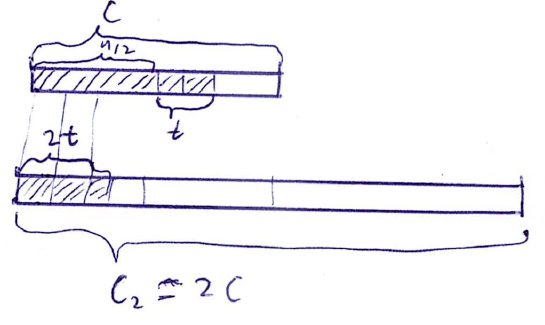
\includegraphics[width=\linewidth]{1-7.png}
\end{minipage}
\end{center}

\end{document}
